%%=============================================================================
%% Onderzoek
%%=============================================================================

\chapter{\IfLanguageName{dutch}{Onderzoek}{Research}}%
\label{ch:onderzoek}

In het voorgaande hoofdstuk werd beschreven hoe het onderzoek te werk zal gaan en welke platformen er onderzocht zullen worden, namelijk Airtable en Google AppSheet. In dit hoofdstuk wordt het daadwerkelijke onderzoek uitgevoerd, waarbij de use case wordt uitgebouwd in elk platform. Bovendien worden de verschillende functionaliteiten van de alternatieven besproken en worden op basis van de criteria vergelijkingen gemaakt tussen elk alternatief en Podio.

\section{Analyse Use Case}

Net zoals bij andere IT-projecten is het belangrijk om eerst een analyse uit te voeren voordat er gestart wordt met ontwikkelen. De analyse voor de use case kan verschillen, afhankelijk van het platform waarvoor ze moet uitgevoerd worden. Aangezien deze studie alternatieven zoekt voor Podio, wordt de analyse fase uitgevoerd in functie van Podio en daarna toegepast op Airtable en Google AppSheet. \\

In Podio wordt een database tabel voorgesteld als een app, die informatie over een bepaald onderwerp bijhoudt. Uit de beschrijving van de use case kan afgeleid worden dat er op zijn minst negen apps aanwezig moeten zijn, namelijk studenten, bedrijven, docenten, stageopdrachten, sollicitaties, richtingen, specialisaties, studentendossiers en evaluaties. \\

Het is belangrijk om in te zien dat studenten en docenten beide personen zijn en dat een bedrijf ook meerdere contactpersonen kan hebben. Om een persistente structuur te hebben, is er dus een 10e app genaamd ‘Contacten’ nodig. Bovendien voorkomt dit ook eventuele redundante data. Een docent kan bijvoorbeeld contactpersoon zijn bij een bedrijf, maar dit kan moeilijk aangetoond worden, aangezien er geen expliciete relatie is tussen ‘Bedrijven’ en ‘Docenten’. Deze persoon zou dus twee keer moeten opgeslagen worden in de databank, wat tegenin de richtlijnen van Podio gaat. \\

Daarnaast moet er ook rekening gehouden worden met het leggen van relaties tussen de verschillende apps. In Podio is het bij 1-op-1 relaties en 1-op-veel relaties beter om de relatie slechts bij één van de twee apps te leggen en bij de andere een calculatie veld te gebruiken. Anders kan er verwarring ontstaan binnenin het platform, indien er bijvoorbeeld een item verwijderd wordt kan de relatie aan één van de kanten nog steeds bestaan. \\

Verder is het belangrijk om na te denken welke automatisaties allemaal toegepast kunnen worden. In dit onderzoek wordt er beperkt tot de volgende;

\begin{itemize}
    \item Automatisch aanmaken van een sollicitatie en linken aan een dossier.
    \item Automatisch aanmaken van een evaluatie en linken aan een dossier.
    \item Automatisch aanmaken van een stageopdracht en linken aan een bedrijf.
    \item Automatisch invullen van de richting wanneer een specialisatie wordt gelinkt aan een stageopdracht.
    \item Automatisch aanmaken van een specialisatie en linken aan een richting.
    \item Dossier automatisch omvormen tot een opgemaakt pdf-bestand.
\end{itemize}

\begin{table}
    \centering
    \caption{\label{tab:Resultaat analyse} }
    \begin{tabular}{ | p{4cm} | p{8cm} | }
        \hline
        \textbf{App} & \textbf{Attributen} \\
        \hline\hline
        Contacten       & (calc.\footnote{calculatie}) ID, voornaam, familienaam, adres, geboortedatum, email, telefoonnummer, (calc.) Bedrijven \\
        Studenten       & (calc.) ID, (rel.\footnote{relatie}) Contact, (rel.) Studierichting, (rel.)  Specialisatie, klasgroep \\
        Bedrijven       & (calc.) ID, naam, adres, email, telefoonnummer, link, (rel.) Contactpersonen, (calc.) Stageopdrachten \\
        Docenten        & (calc.) ID, rol, (rel.) Studierichting \\
        Stageopdrachten & (calc.) ID, titel, (rel.) Bedrijf, beschrijving, (rel.) Richting, (rel.) Specialisaties, periode, aantal-studenten, (rel.) Toegewezen-aan \\
        Sollicitaties   & (calc.) ID, (rel.) Student, (rel.) Bedrijf, datum-gesprek, alleen/medestudent, (rel.) Medestudent, resultaat, opmerking \\
        Richtingen      & (calc.) ID, naam, afkorting, status, (calc.) Specialisaties \\
        Specialisaties  & (calc.) ID, naam-specialisatie, (rel.) Richting \\
        Dossiers        & (calc.) ID, Titel, (rel.) Student, (rel.) Begeleider, (rel.) Sollicitaties, (rel.) Evaluaties, (rel.) Toegewezen-stageopdracht, (calc.) Score \\
        Evaluaties      & (calc.) ID, datum, (rel.) Student. \\
        \hline
    \end{tabular}
\end{table}

Ten slotte kan het resultaat van de analyse fase terug gevonden worden in tabel \ref{tab:Resultaat analyse}. Nu deze fase voltooid is, kan er gestart worden met het ontwikkelen in Podio, Airtable en Google AppSheet. Vervolgens wordt voor elk van de platformen nogmaals de criteria overlopen en wordt er toegelicht hoe goed elk platform eraan voldoet. \\

\newpage



% PODIO __________________________________________________________________________________________________________________________
\section{Podio} 

Vooraleer het bouwproces wordt toegelicht is het belangrijk om nog eens de structuur van Podio op te frissen. In Podio wordt een use case of project weergegeven aan de hand van een workspace. Deze workspace bevat één of meerdere apps die een template voorzien voor een bepaald onderdeel. Een template wordt gebruikt om een item van de app op te bouwen en is een samenstelling van velden zoals een tekstveld, datumveld of calculatieveld. Vanuit een database-perspectief kan een workspace dus gezien worden als de database, een app als een tabel, een template als de kolommen van de tabel en een item als een rij in de tabel. \\

In Podio is de eerste stap van het ontwikkelingsproces dus het aanmaken van de workspace waarin alles gebouwd zal worden. De ‘Activity’ app, zie figuur \ref{fig:meth_podio_workspace}, wordt standaard aangemaakt bij het creëren van een workspace en bevat een overzicht van wat er zich allemaal afspeelt. Indien iets wordt aangepast, wordt dit weergegeven in de tijdslijn, samen met de persoon die het heeft aangepast en wanneer de aanpassing verricht werd. Daarnaast wordt ook een kalendertegel en een lijsttegel, met taken die zelf kunnen toegevoegd worden, voorzien. Bovendien is er de optie om zelf tegels toe te voegen die data uit de workspace kunnen weergeven. \\

\begin{figure}[h]
    \centering
    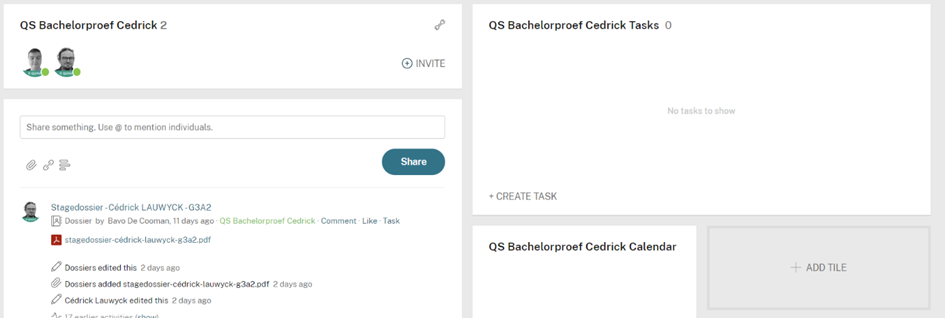
\includegraphics[width=0.85\textwidth]{methodologie/Podio_workspace.png}
    \caption{'Activity' app in een Podio workspace.}
    \label{fig:meth_podio_workspace}
\end{figure}

Nadat de workspace is aangemaakt, kan voor elk onderwerp uit de analyse een app aangemaakt worden. Het is voordeliger om eerste alle apps aan te maken vooraleer de attributen worden toegevoegd, want er kunnen namelijk geen relaties gelegd worden naar iets dat nog niet bestaat. Dit kan eenvoudig gedaan worden door op de ‘Add App’-knop te klikken, waarna een venster getoond wordt die vraagt om de naam van de app, de naam van een item en een icoon voor de app. Voor de benamingen wordt door Quivvy vaak meervoud en enkelvoud gebruikt, ter illustratie: de ‘Contacten’ app heeft ‘Contact’ als naam van het item. Het icoon daarentegen kan gekozen worden uit een uitgebreide lijst van iconen. Het uiteindelijke resultaat van deze stap wordt weergegeven in figuur \ref{fig:meth_podio_lijstApps}. \\

\begin{figure}[h]
    \centering
    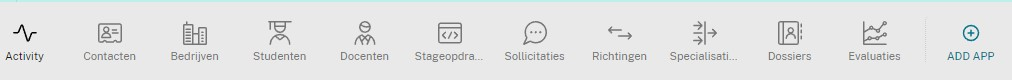
\includegraphics[width=0.85\textwidth]{methodologie/Podio_lijstApps.jpg}
    \caption{Aangemaakte apps in de Podio workspace.}
    \label{fig:meth_podio_lijstApps}
\end{figure}

Eens alle apps aangemaakt zijn, is de fundering van de use case afgewerkt. Nu kan er overgegaan worden tot het instellen van de verschillende attributen en relaties. Dit is mogelijk in twee simpele klikken, namelijk door naar de app te navigeren en vervolgens via het ‘moersleutel’-icoontje de verschillende instellingen te openen. Daarna kan via een derde klik de template van de app bewerkt worden. Zoals eerder vermeld is een template een samenstelling van verschillende types velden die Podio voorziet. Voor de use case wordt dus elk voor elk attribuut van de app een veld toegevoegd. Ter illustratie wordt in figuur \ref{fig:meth_podio_dossierTemplate} de uitgewerkte template voor de 'Dossiers' app van de use case weergegeven. Eerst een vooral werd een calculatieveld toegevoegd voor de ID van het dossier. In dit veld komt het low-code gedeelte van Podio aan bod, het veld accepteert namelijk JavaScript en kan op allerlei manieren gebruikt worden. De laatste lijn in het calculatie veld is wat er uiteindelijk wordt weergegeven, daaronder is ook een preview zichtbaar. In het geval van een dossier wordt een stuk tekst samengevoegd met de ID van de gelinkte student. Vervolgens wordt een simpel tekstveld gebruikt voor de titel van het dossier, gevolgd door twee relatievelden om de student en begeleider te linken. Daarna wordt een categorieveld ingevoegd met de opties `Evaluatie` en `Sollicitatie`, dit zal later gebruikt worden voor het toevoegen van een evaluatie of sollicitatie via automatisaties. Podio voorziet namelijk geen 'Button' velden, om die reden wordt een categorie veld gebruikt als workaround. Verder worden nog twee relatievelden toegevoegd en nog een calculatieveld waarin de totaalscore van de evaluaties wordt uitgerekend en weergegeven. Het is belangrijk om te vermelden dat er voor elk veld een set van opties beschikbaar is, om bijvoorbeeld het veld verplicht te maken of om het aantal relaties in een relatieveld te beperken. \\

\begin{figure}[h]
    \centering
    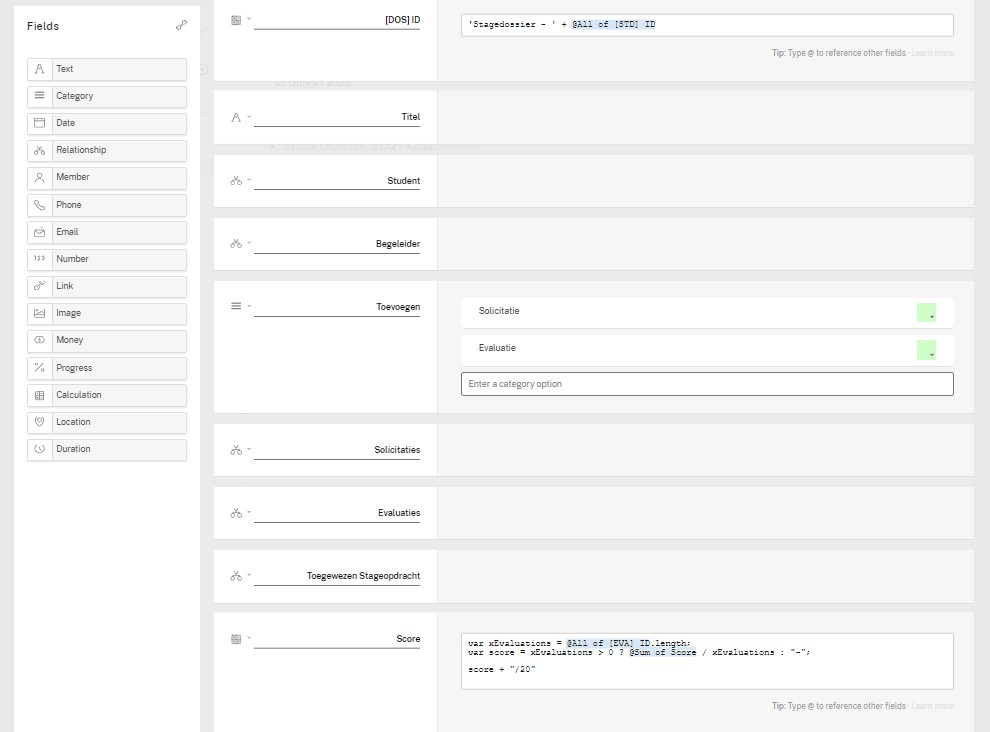
\includegraphics[width=\linewidth]{methodologie/Podio_dossierTemplate.jpg}
    \caption{Uitgewerkte template van de 'Dossier' app.}
    \label{fig:meth_podio_dossierTemplate}
\end{figure}

Om de data mooi weer te geven wordt als extra ook de layout aangepast. Podio voorziet standaard vijf verschillende layouts, namelijk 'Badge', 'Table', 'Card', 'Activity' en 'Calender', verder kunnen ook nog filters ingesteld worden op de attributen van een app. Eens alles geconfigureerd is naar keuze kan ten slotte de weergave als view opgeslagen worden. In figuur \ref{fig:meth_podio_badgeLayout} is een voorbeeld van de badge layout te zien. Bovendien kan men voor elke app via de 'Layout options' selecteren welke velden men wil weergeven op een individuele badge. \\

\begin{figure}[h]
    \centering
    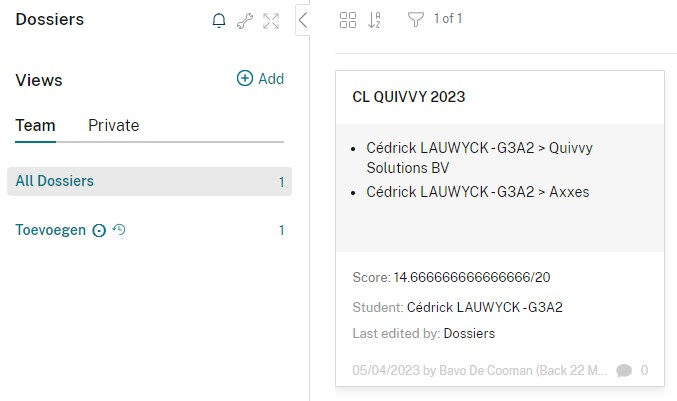
\includegraphics[width=\linewidth]{methodologie/Podio_badgeLayout.jpg}
    \caption{Badge layout in Podio.}
    \label{fig:meth_podio_badgeLayout}
\end{figure}

De volgende stap is om de automatisaties of workflows toe te voegen, dit gebeurt via Citrix Podio Workflow Automation\footnote{voorheen Globiflow genoemd.} (CPWA), een geavanceerde workflow automation tool gemaakt voor Podio. Door naar de instellingen van een willekeurige app te navigeren en vervolgens door te klikken op `workflow automations`, wordt men omgeleid naar een externe pagina waar automatisaties kunnen worden ingesteld. Eerst en vooral is het belangrijk om onderaan de pagina op de 'Refresh from Podio' knop te klikken, deze zorgt er namelijk voor dat de laatst opgeslagen configuratie van de Podio workspace wordt opgehaald. Nu alle apps en bijkomende velden aanwezig zijn, kunnen er workflows aangemaakt worden. Deze bevatten een trigger, een set van filters en een set van acties die worden uitgevoerd. Er zal dus voor elke automatisatie in de analyse, een workflow aangemaakt worden. Een handige feature van CPWA, is dat het voor elke workflow ook een verkorte versie of recept weergeeft. Bovendien wordt ook een schatting weergegeven van hoeveel minuten er bespaard worden door de workflow uit te voeren. \\

In figuur \ref{fig:meth_podio_workflow} is terug een uitgewerkt voorbeeld te zien, namelijk het omvormen van een dossier tot pdf-bestand. De trigger voor deze workflow is het updaten van een dossier, in de filters wordt dit dan verfijnd tot het updaten van het 'Verwerken' veld. Eens dit op 'Omzetten naar PDF' wordt gezet, zal de flow verdergaan naar de acties, bij een andere waarde wordt de flow beëindigd. Bij de eerste actie wordt een variabele opgeslagen met het jaartal van de creatiedatum van het dossier, deze zal dan later gebruikt worden in de template voor het omvormen naar pdf. Vervolgens wordt de data van enkele referenties opgehaald, namelijk de informatie over de student, studierichting en het bedrijf. Daarna komt het omzetten naar pdf-bestand, Een template kan volledig zelf opgebouwd worden met alle nodige informatie uit Podio. Bovendien is het ook mogelijk om een footer en header in te stellen, voor de use case wordt in de footer bijvoorbeeld informatie over HOGENT weergegeven. Er hoeft geen actie toegevoegd te worden om de gemaakte pdf aan het item zelf te hangen, want dit zit namelijk inbegrepen in de actie. Indien een gebruiker het bestand zou willen doormailen, kan dat eenvoudig door vanuit deze workflow een andere workflow te activeren en vervolgens de gegenereerde pdf mee te geven. De voorlaatste stap van automatisatie is het `Dossier` item terug updaten om het 'Toevoegen' veld terug op leeg te zetten. Ten slotte worden nog enkele acties toegevoegd om de referenties die eerder werden opgehaald terug op te ruimen, eens dit gebeurt is, is de workflow afgewerkt. \\

\begin{figure}[h]
    \centering
    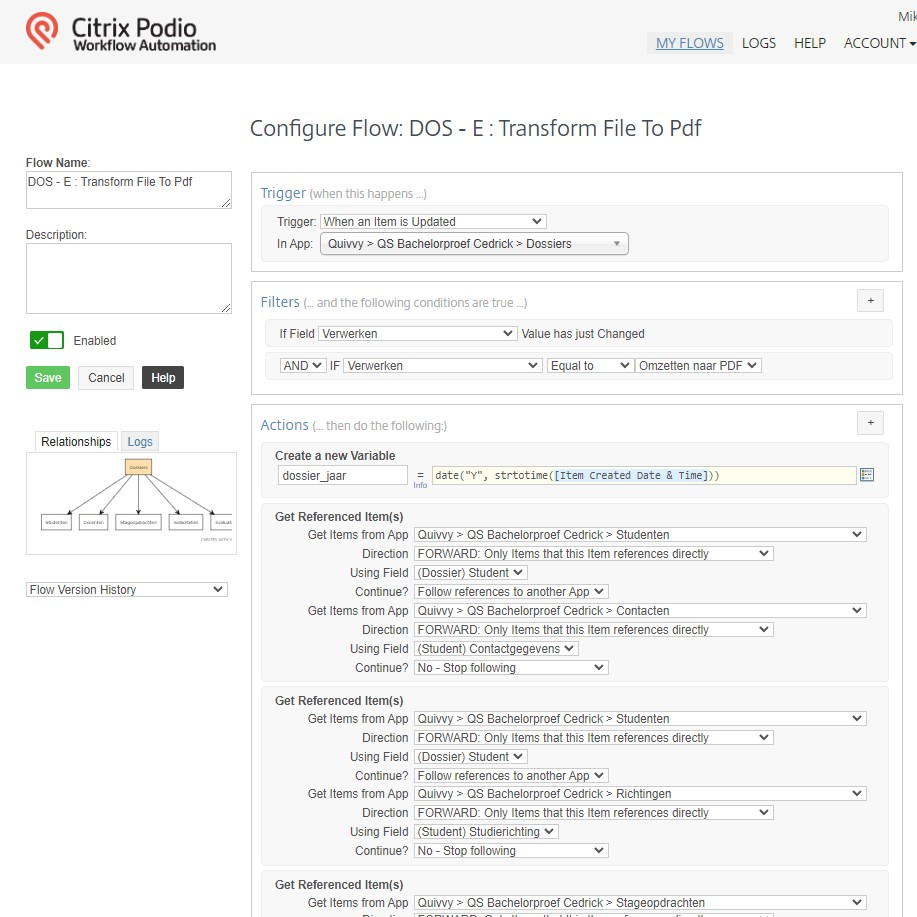
\includegraphics[width=0.85\textwidth]{methodologie/Podio_workflow.jpg}
    \caption{Workflow in Citrix Podio Workflow Automation.}
    \label{fig:meth_podio_workflow}
\end{figure}

Nu de use case is voltooid in Podio, is het belangrijk om de criteria eens door te nemen en kort te evalueren hoe goed het platform zelf presteert. Allereerst is het heel eenvoudig om relaties te leggen via het relatieveld, hoewel er wel altijd nagedacht moet worden aan welke kant de relatie wordt gelegd. Ten tweede kunnen workflows ook gemakkelijk worden ingesteld. Alles heeft een duidelijke benaming, waardoor zelfs lange reeksen van acties eenvoudig te begrijpen zijn. Verder zijn calculaties heel krachtig en flexibel, omdat het type veld JavaScript ondersteund. Bovendien biedt Podio een prettige gebruikerservaring. De verschillende knoppen en functies zijn gemakkelijk te begrijpen en kunnen met slechts één tot vier klikken worden bereikt. \\

Het uitbouwen van de use case is echter niet zonder problemen verlopen. Bijvoorbeeld, het instellen van de 'layout options' voor een badge moest vaak twee keer worden toegepast, omdat ze de eerste keer niet werden opgeslagen in het systeem. \\

\newpage



% AIRTABLE __________________________________________________________________________________________________________________________
\section{Airtable}

Nu de use case uitgewerkt is in Podio kan overgegaan worden naar het eerste potentiële alternatief, Airtable. De structuur van Airtable is gelijkaardig aan die van Podio, ook hier wordt weer gewerkt met workspaces. In een workspace kan dan een base of database worden aangemaakt, deze zal alle data van de use case omvatten. Verder bestaat een base uit zogenaamde `Tables` of tabellen, die vergelijkbaar zijn met apps uit Podio of dus met een tabel in een database. Voor elk onderwerp uit de analyse wordt dus een tabel toegevoegd, de attributen of kolommen zullen later ingesteld worden. Bij het aanmaken wordt er gekozen om een lege tabel te creëren. Daarnaast voorziet Airtable net zoals Podio ook de optie om een tabel aan te maken gebaseerd op een csv-bestand\footnote{simpel bestandsformaat om tabulaire data op te slaan}. Verder kan er ook data uit verschillende andere bronnen zoals Google Drive, Salesforce of Jira Server,$\ldots$ gehaald worden, wat niet standaard ingebouwd zit in Podio. \\

Wanneer alle tabellen aangemaakt zijn, ziet de structuur eruit zoals in figuur \ref{fig:meth_airtable_tables}. Airtable maakt gebruik van een tabblad structuur, waardoor het afwisselen tussen tabellen zeer vlot gaat. De data laadt ook aanzienlijk sneller in vergelijking met Podio, dit zorgt dan weer voor een zeer aangename gebruikerservaring. \\

\begin{figure}[h]
    \centering
    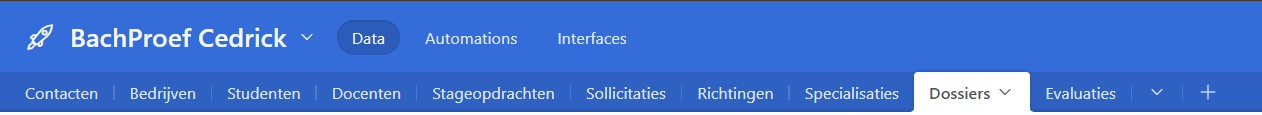
\includegraphics[width=0.85\textwidth]{methodologie/Airtable_tables.jpg}
    \caption{Tables in Airtable.}
    \label{fig:meth_airtable_tables}
\end{figure}

Eens de vorige stap voltooid is, kunnen de attributen per tabel worden ingesteld. In Airtable stelt elke kolom van een tabel een attribuut voor. Om die redenen zijn er dus ook verschillende soorten velden, zoals een `Email` veld om een e-mail bij te houden of een 'Phone' veld om een telefoonnummer bij te houden. Een klein verschil met Podio is dat Airtable geen speciaal veld voorziet om een adres op te slaan. Dit is toch wel belangrijk en maakt het bijhouden van een adres minder eenvoudig, aangezien dit dus door een gewoon tekstveld moet gebeuren. \\

De twee belangrijkste types velden zijn het `Relationship` veld en het `Formula` veld. Zoals de naam impliceert, wordt het `Relationship` veld gebruikt om, net zoals in Podio, relaties te leggen tussen de verschillende tabellen. Relaties op zich zijn goed uitgewerkt in Airtable, in tegenstelling tot Podio worden ze direct aan beide kanten toegevoegd. Dit betekent dat als er bijvoorbeeld in de `Specialisaties` tabel een link gelegd wordt naar `Richtingen`, dan zal er ook automatisch een relatieveld worden toegevoegd in de tabel 'Richtingen'. Bovendien kan er net zoals in Podio gekozen worden of het veld één of meerdere referenties mag bevatten. Verder heeft Airtable ook nog het `Lookup` veld, waarmee een waarde uit een andere tabel kan worden weergegeven. Om dit in Podio te bereiken zou een calculatieveld gebruikt moeten worden. \\

Het 'Formula' veld is vergelijkbaar met een calculatieveld in Podio. Hiermee kunnen aangepaste formules gemaakt worden op basis van andere velden in dezelfde tabel. Bovendien ondersteunt het veld een groot aantal functies en operatoren, waaronder wiskundige, logische en tekstfuncties. Verder is ook conditionele logica zoals een 'if-else' structuur mogelijk. Toch is dit veld minder krachtig dan het calculatieveld in Podio, omdat het aantal functies en mogelijkheden beperkter is. Kortom is het dus een krachtig hulpmiddel voor gegevensverwerking binnen Airtable.  In de use case wordt dit type veld vooral gebruikt om de ID's van de verschillende tabellen te berekenen. \\

In figuur \ref{fig:meth_airtable_dossiersTable} is de uitgewerkte tabel voor de 'Dossiers' weergegeven, waarvan structuur van de opzet nagenoeg dezelfde is als die in Podio, op enkele verschillen na. Zo wordt voor de totaalscore bijvoorbeeld gebruik gemaakt van een ander soort veld dan het `Formula` veld. In tegenstelling tot het calculatieveld in Podio ondersteunt het `Formula` veld geen loops, in plaats daarvan voorziet Airtable het `Roll-up` veld. Hiermee kan een lijst met waarden, afkomstig uit een relatie, worden verwerkt. Zo wordt voor de totaalscore de som gemaakt van elke score bij de evaluaties en daarna gedeeld door 20. \\ 

\begin{figure}[h]
    \centering
    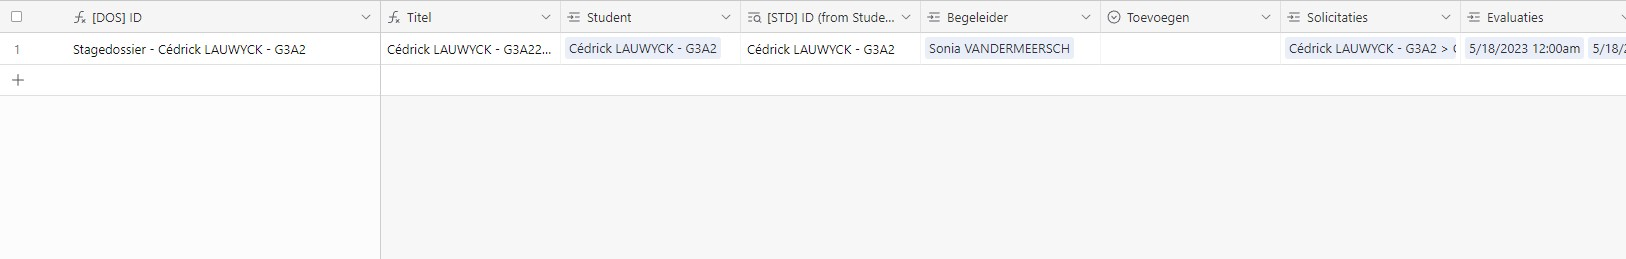
\includegraphics[width=0.85\textwidth]{methodologie/Airtable_tableDossier.jpg}
    \caption{Uitgewerkte 'Dossiers' table in Airtable.}
    \label{fig:meth_airtable_dossiersTable}
\end{figure}

Net zoals in Podio kan de data op verschillende manieren weergegeven worden. De standaardweergave is een gewone tabel, maar er kan bijvoorbeeld ook voor een 'Grid' layout gekozen worden. Deze is gelijkaardig aan de 'Badge' layout in Podio. Verder kan net zoals in Podio geselecteerd worden welke velden er moeten worden weergegeven op een individuele card. Dit via een enkele klik op de 'Customize Cards' knop. \\

Na het instellen van de attributen, kan overgegaan worden tot de laatste stap in het bouw proces, namelijk automatisaties of workflows invoegen. In tegenstelling tot Podio, zitten deze wel ingebouwd in het platform en zijn ze gemakkelijk te bereiken via één simpele klik. In figuur \ref{fig:meth_airtable_automations} is te zien hoe ze zeer overzichtelijk worden weergegeven. Verder toont de figuur ook hoe een eenvoudige workflow is opgebouwd. In contrast met Podio is er geen apart gedeelte voor filters, maar zitten deze ingebouwd in de configuratie van de trigger,  daarna volgen direct de acties. Bovendien is er ook de optie om een workflow uit te testen, wat in Podio niet het geval is. \\

\begin{figure}[h]
    \centering
    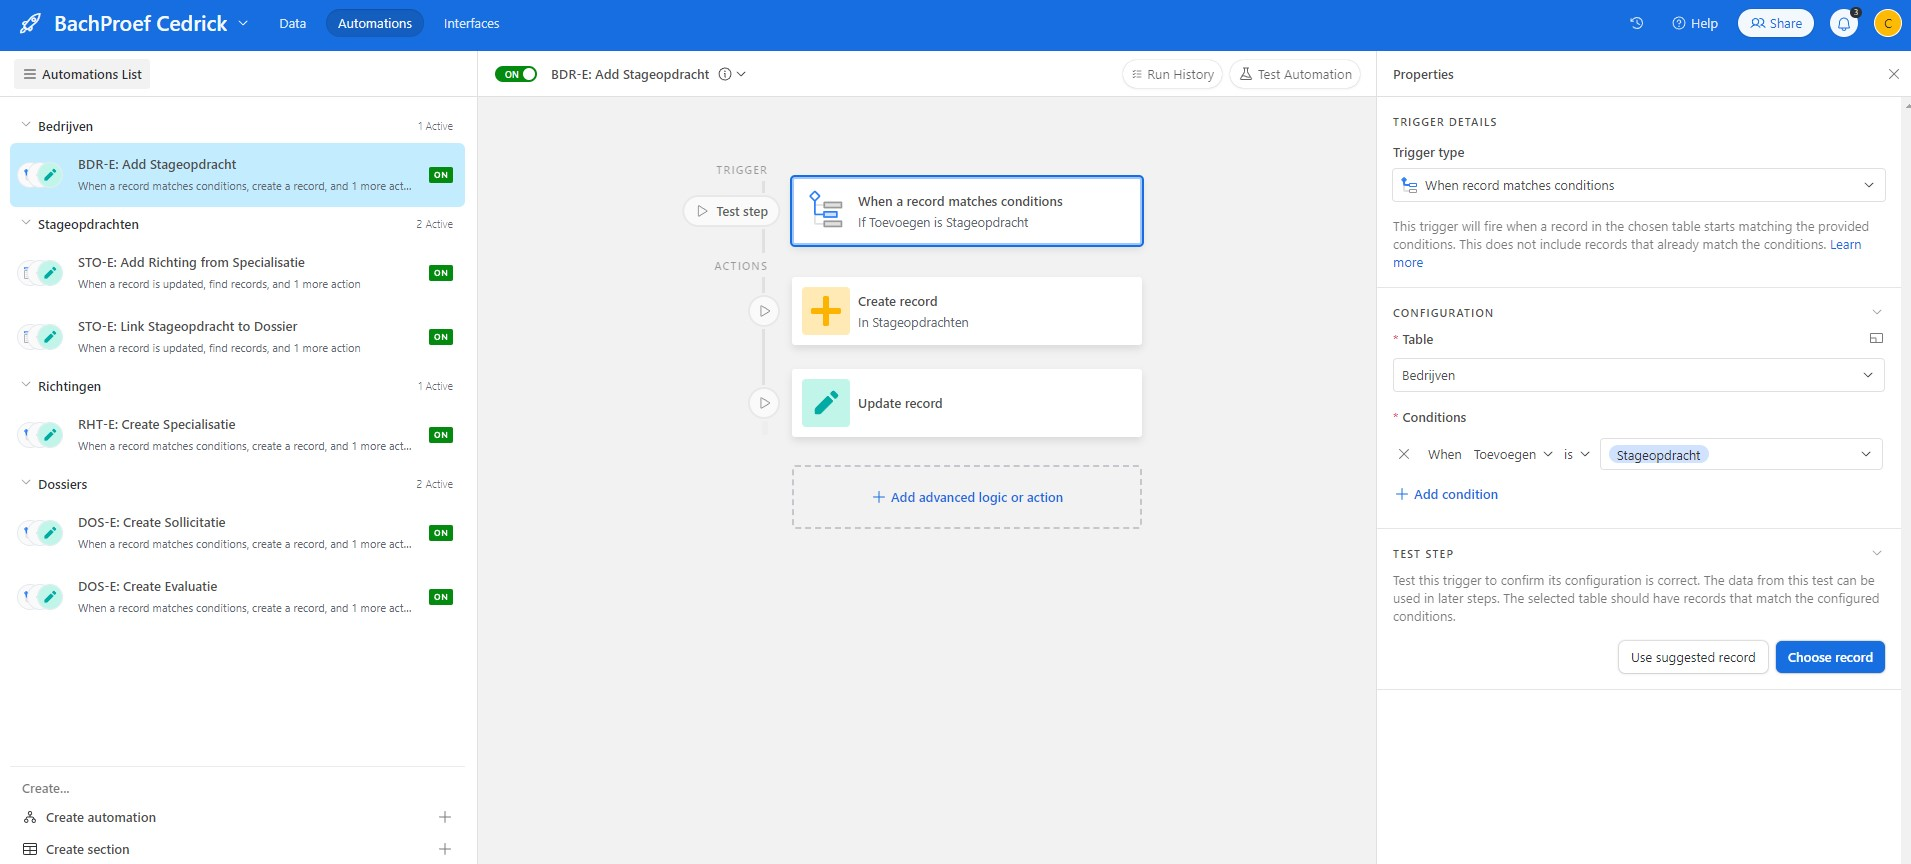
\includegraphics[width=0.85\textwidth]{methodologie/Airtable_automations.jpg}
    \caption{Overzicht van automatisaties in Airtable.}
    \label{fig:meth_airtable_automations}
\end{figure}


Het omzetten tot pdf-bestand daarentegen is in Airtable minder eenvoudig dan als in Podio. Airtable voorziet in automatisaties namelijk geen optie om een pdf-bestand op te stellen, maar hier moet dit gebeuren via een extensie. Eerst en vooral is het belangrijk te vermelden dat de optie om extensies toe te voegen, ingebouwd zit in Airtable, wat in Podio niet het geval is. Er zijn verschillende extensies die het opmaken van een pdf-bestand verwezenlijken, zo heb je onder andere de `Page Designer` extensie, die ontwikkeld is door Airtable zelf. Hiermee kunnen mooie templates opgesteld en ingevuld worden met data uit de tabellen. Deze extensie beperkt zich wel tot een enkele pagina, wat dus niet bij elke use case het geval is. Uiteindelijk werd voor deze use case gekozen om gebruik te maken van de `PDF Generator API` extensie. Ook hier wordt vooraf een simpele template opgesteld om vervolgens op te vullen met de gewenste velden uit de 'Dossiers' tabel. Ten slotte hoeven enkel nog de records die geconverteerd moeten worden, geselecteerd worden en kan een pdf-bestand gegenereerd worden. Dat pdf-bestand wordt dan toegevoegd in het `Attachments` veld van de records, zoals weergegeven in figuur \ref{fig:meth_airtable_dossiersAttachments}. Hoewel hier dus geen automatisatie werd aangemaakt, is het wel degelijk mogelijk om een extensie uit te voeren via een automatisatie. Via de betaalde 'Pro' versie van Airtable kunnen in automatisaties scripts toegevoegd worden die het gebruik van extensies toelaten.  \\

\begin{figure}[h]
    \centering
    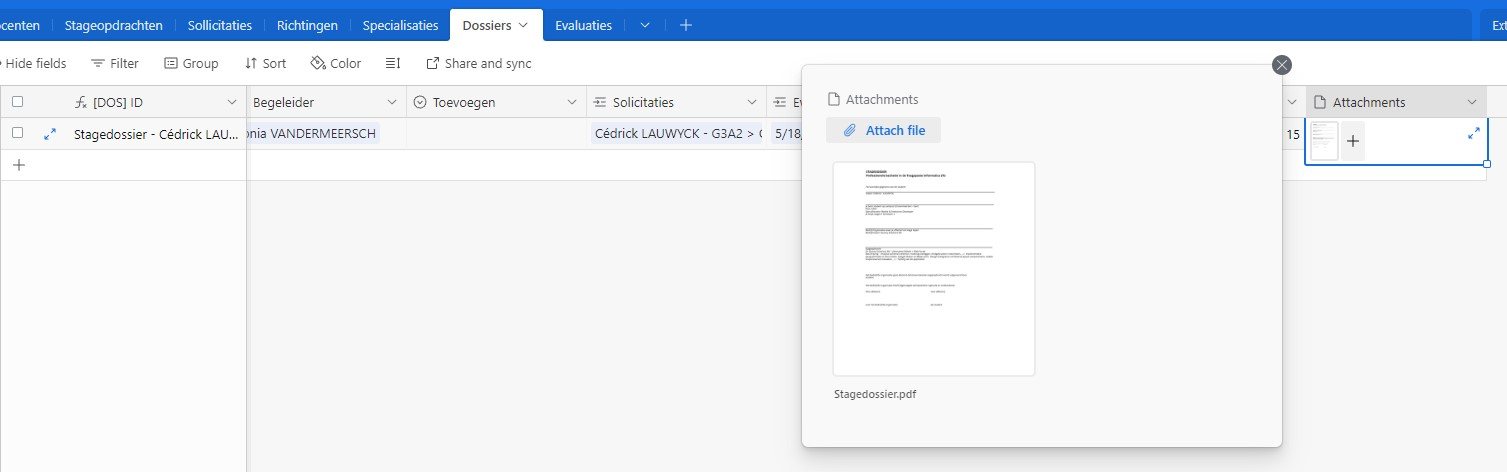
\includegraphics[width=0.85\textwidth]{methodologie/Airtable_dossiersAttachments.jpg}
    \caption{Pdf-bestand toegevoegd aan attachments veld in 'Dossiers' table na het uitvoeren van de workflow.}
    \label{fig:meth_airtable_dossiersAttachments}
\end{figure}

Ten slotte kan dus besloten worden dat het perfect mogelijk is om de use case uit te bouwen in Airtable. Ten eerste is het leggen van onderlinge relaties tussen verschillende tabellen zeer goed uitgewerkt, beter dan in Podio om dat er minder over nagedacht moet worden aan welke kant de relatie gelegd wordt. Op gebied van calculaties presteert Airtable minder goed dan Podio, omdat het een beperkter aantal mogelijkheden bied. Aan de andere kant is er voor Podio wel iets meer technische kennis over JavaScript nodig, terwijl dit in Airtable niet het geval is. Vervolgens is de gebruikerservaring in Airtable heel wat aangenamer dan die van Podio. Desondanks het feit dat in het algemeen een gelijkaardig aantal klikken nodig zijn om een bepaald doel te bereiken, wordt in Airtable nagenoeg geen tijd gebruikt voor het afwisselen tussen tabellen en inladen van de data, wat te danken is aan hun tabblad-structuur. Bovendien voorziet het platform ook een korte tutorial in het begin, waardoor een gebruiker gemakkelijk op weg geraakt. Verder is de gebruikersinterface of UI zeer mooi opgesteld. De belangrijkste functionaliteiten zijn eenvoudig te bereiken en de gebruiker wordt niet overrompeld door informatie. Een klein nadeel is wel dat er geen overzicht is voor de verschillende activiteiten die gebeuren binnen een workspace. Ten slotte werden tijdens het uitbouwen van de use case geen problemen tegengekomen, alles verliep vlot en de functionaliteiten werkten zoals behoort. \\

\newpage



% APPSHEET __________________________________________________________________________________________________________________________
\section{Google AppSheet} 

Nu ook Airtable onderzocht werd, kan worden overgegaan tot het tweede en laatste potentiële alternatief, namelijk Google AppSheet. Eerst en vooral is de structuur van Appsheet opmerkelijk anders dan die van Podio of Airtable. Zoals weergegeven in figuur \ref{fig:meth_appsheet_structuur}, maakt het platform namelijk geen gebruik van workspaces en splitst het bovendien projecten op in databases en applicaties. Alhoewel dit voor een slechtere gebruikerservaring zorgt, omdat er vaak moet afgewisseld worden tussen de twee delen, heeft dit wel als voordeel dat een enkele database gebruikt kan worden door meerdere applicaties. Bij het aanmaken van een app is er net zoals bij Podio en Airtable de optie om data te importeren van een externe bron, namelijk de Google Drive van de gebruiker. Indien er voor gekozen wordt een blanco app aan te maken, zal Appsheet automatisch ook een achterliggende database creëren. \\

\begin{figure}[h]
    \centering
    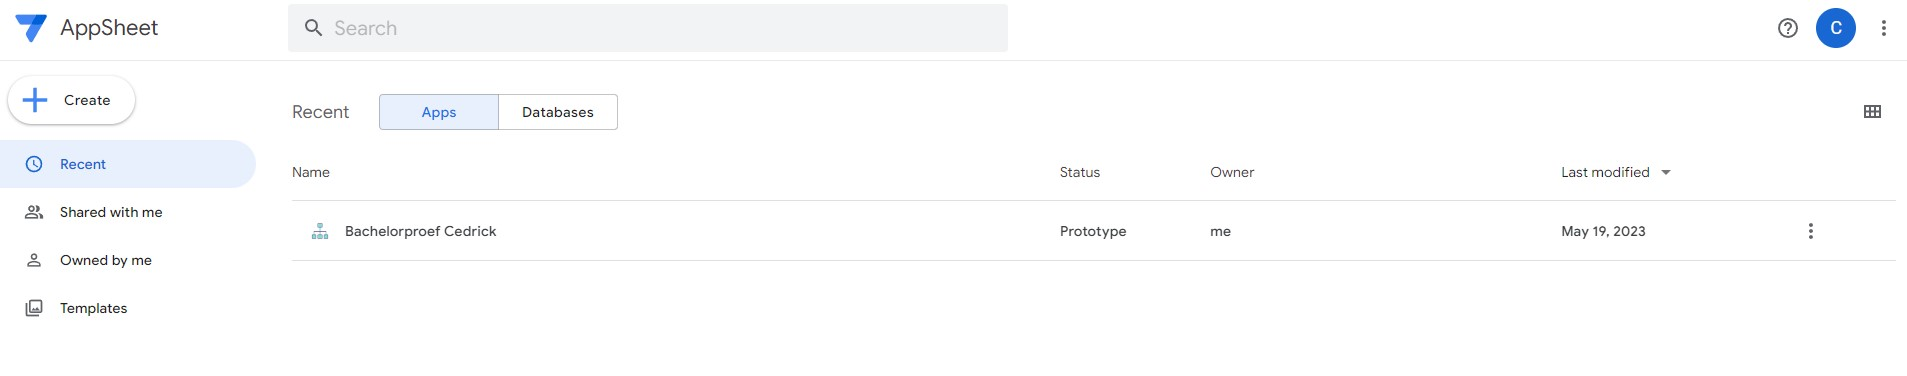
\includegraphics[width=0.85\textwidth]{methodologie/Appsheet_structure.jpg}
    \caption{Structuur van AppSheet.}
    \label{fig:meth_appsheet_structuur}
\end{figure}

% uitleg structuur applicatie
Nadat de applicatie aangemaakt is, moet eerst de database correct geconfigureerd worden. In figuur \ref{fig:meth_appsheet_database} is te zien dat net zoals Airtable ook AppSheet met 'Tables' of tabellen werkt. Voor elk onderwerp uit de analyse wordt dus een tabel aangemaakt. Verder stellen ook de kolommen van de tabel terug de attributen voor, dus wordt voor elk attribuut een kolom aangemaakt. Net zoals bij Airtable en Podio zijn er een groot aantal verschillende velden waaruit gekozen kan worden die het type van een attribuut voorstellen. In het algemeen bevat AppSheet zelfs meer types velden dan de vorige platformen. Toch ontbreekt er een zeer belangrijk veld, er is namelijk geen calculatie of 'Formula' veld. In Appsheet kunnen berekeningen of tekstverwerkingen niet ingesteld worden in de database zelf, maar gebeurt dit in het applicatie gedeelte, deze worden dus pas achteraf ingesteld. Daarnaast moeten de verschillende tabellen wel nog gelinkt worden met elkaar, dit gebeurt via het `Relationship` veld, dat zeer eenvoudig ingesteld kan worden. Verder heeft ook AppSheet een 'Look-up' veld dat toelaat om data uit een andere tabel weer te geven. \\

\begin{figure}[h]
    \centering
    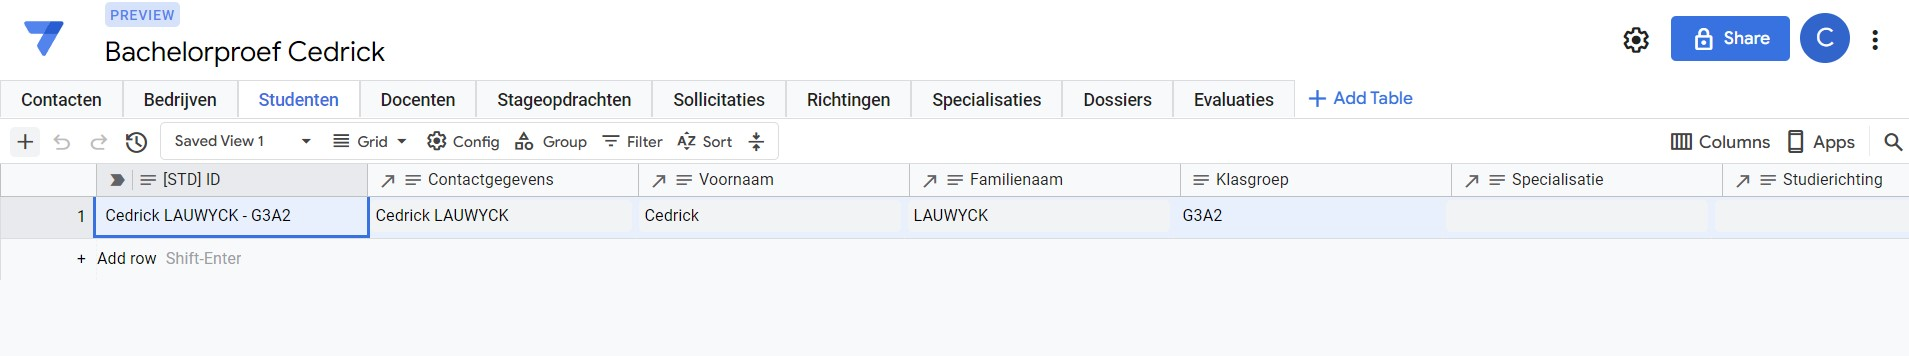
\includegraphics[width=0.85\textwidth]{methodologie/Appsheet_database.jpg}
    \caption{Database in AppSheet.}
    \label{fig:meth_appsheet_database}
\end{figure}

Vervolgens kan overgegaan worden naar het applicatie gedeelte van het bouwproces, waar de formules worden toegevoegd. De structuur van dit deel wordt weergegeven in figuur \ref{fig:meth_appsheet_views} en gaat als volgt. Aan de rechterkant van het scherm wordt altijd een preview van de gebouwde applicatie getoond, de resterende ruimte wordt dan ingevuld met de verschillende configuratie opties. Om data weer te geven in de app, moet eerst een view aangemaakt en toegevoegd worden aan het menu. Een view omvat één tabel uit de database en geeft zijn data weer. Dit kan als verschillende vormen gebeuren, zoals als een gewone lijst of als een dashboard. Bovendien kan data die een 'Address' veld bevat ook weergegeven worden op een map door de ingebouwde Google Maps integratie die AppSheet voorziet. Uiteindelijk wordt dus voor elke tabel die werd aangemaakt in de vorige stappen een view gecreëerd. \\

\begin{figure}[h]
    \centering
    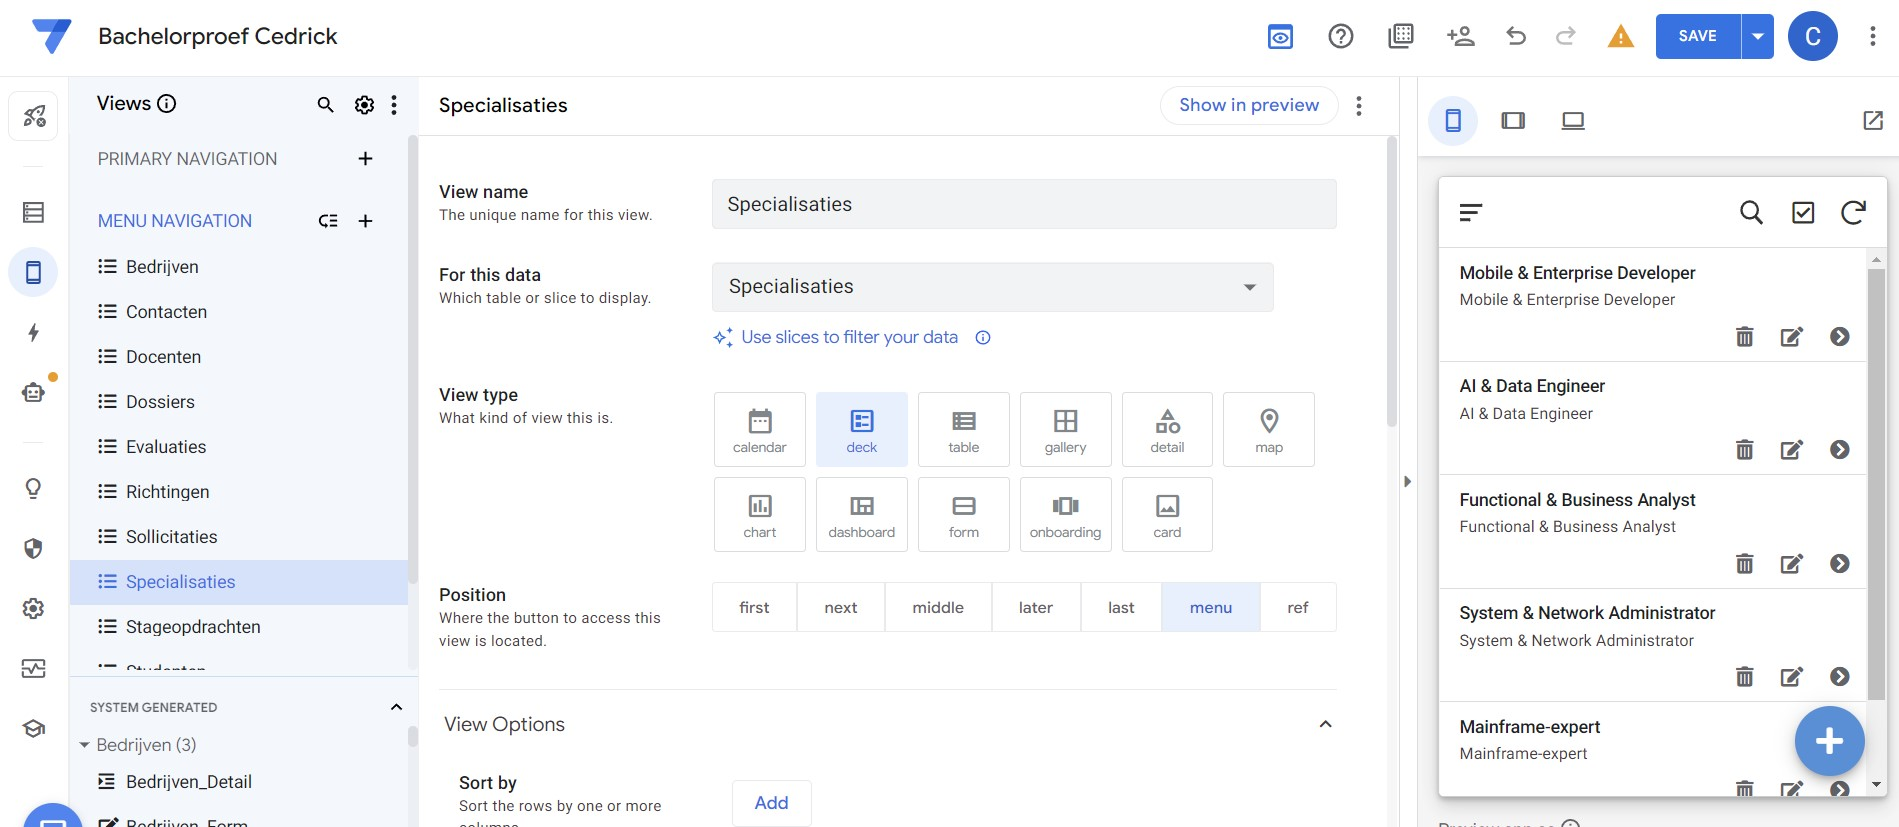
\includegraphics[width=0.85\textwidth]{methodologie/Appsheet_views.jpg}
    \caption{Weergave van data in AppSheet.}
    \label{fig:meth_appsheet_views}
\end{figure}

Nu kunnen formules toegevoegd worden. De eerste stap hierbij is om bij elke tabel op de 'Regenerate schema' knop te klikken. Dit zorgt ervoor dat de verschillende database schema's in de applicatie up-to-date zijn met diegene in de database. Daarna kunnen de nodige formules ingevuld worden, deze zijn vergelijkbaar met formules in Microsoft Excel. In tegenstelling tot Podio kan in Appsheet elk veld als calculatieveld gebruikt worden. In figuur \ref{fig:meth_appsheet_formulas} is te zien hoe bij het invoeren van de calculaties er ook een `Expression Assistant` is die verschillende soorten voorbeeldformules weergeeft en ook de mogelijkheid bied om ze te testen. Daarnaast is er ook een 'Data Explorer' waarmee men gemakkelijk de nodige attributen kan invoeren. In het algemeen is het calculatieveld hier wel weer beperkter dan in Podio. Uiteindelijk is het nog belangrijk om te vermelden dat berekeningen in AppSheet geen conditionele logica ondersteunen, wat toch wel een redelijk groot nadeel is. \\

\begin{figure}[h]
    \centering
    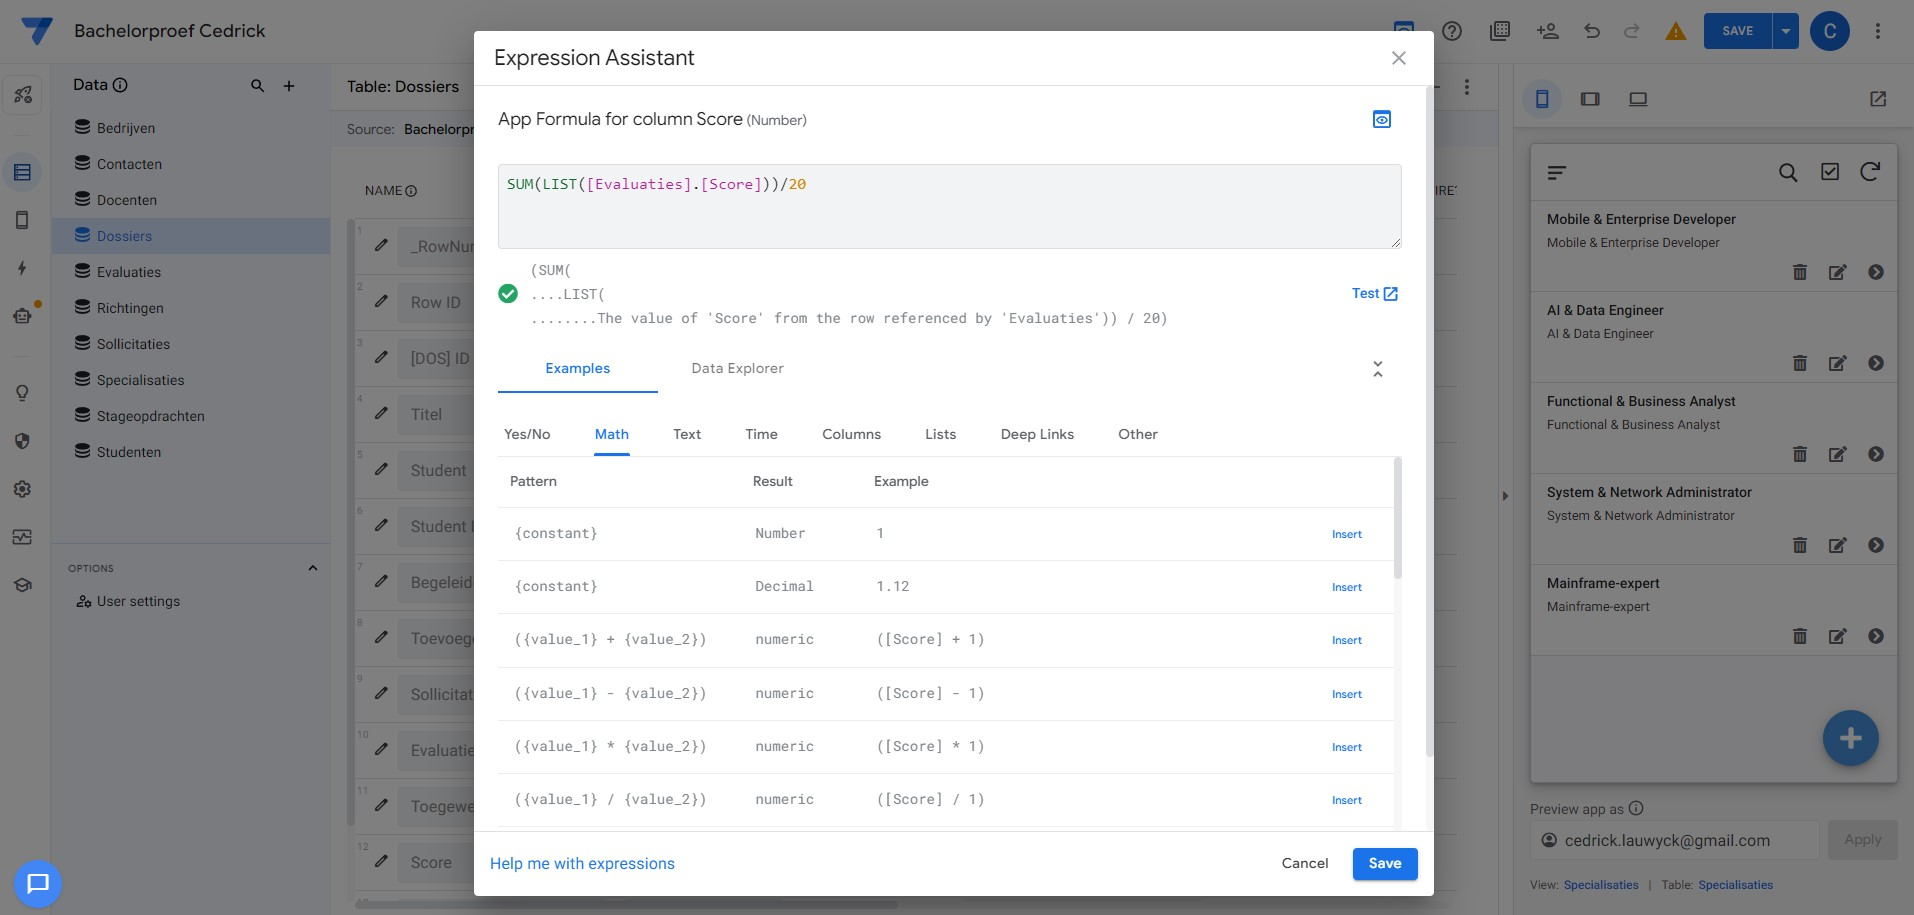
\includegraphics[width=0.85\textwidth]{methodologie/Appsheet_formulaAssistant.jpg}
    \caption{Formules met `Expression Assistant` in Appsheet.}
    \label{fig:meth_appsheet_formulas}
\end{figure}

Een belangrijke opmerking bij Appsheet is dat het aanvullen van de database met gegevens in het applicatiegedeelte gebeurt. Hoewel de mogelijkheid bestaat om rijen toe te voegen in het database gedeelte, zullen op die manier de verschillende formules niet worden toegepast op de data. \\


% automatisaties
Nu kan terug overgegaan worden tot de laatste stap, automatisaties. In Appsheet hoeft enkel de automatisatie voor het omzetten naar pdf-bestand aangemaakt worden. De andere workflows zijn namelijk overbodig, omdat Appsheet al automatisch de mogelijke gelinkte velden invult indien we op de 'Add'-knop klikken in de applicatie. Automatisaties zijn gemakkelijk te bereiken via een enkele klik op het `robot`-icoontje. Zoals te zien is in figuur \ref{fig:meth_appsheet_automations} wordt een automatisatie in AppSheet gedefinieerd door een zogenaamde `bot`, deze hebben hetzelfde concept als in Podio en Airtable, ze hebben namelijk een set van acties die worden uitgevoerd eens een bepaalde trigger geactiveerd wordt. Voor de use case wordt een bot gezet op de tabel dossiers, met als trigger een verandering in de kolom 'Toevoegen'. Vervolgens wordt een actie toegevoegd om het dossier om te zetten naar een pdf-bestand. In tegenstelling tot Airtable zit deze functionaliteit net zoals in Podio ingebouwd in AppSheet. Een nadeel is wel dat de gegenereerde pdf achteraf niet zomaar aan het dossier kan worden toegevoegd. Het wordt namelijk opgeslagen op een aparte plaats, zoals Google Drive of OneDrive. Om het bestand te linken aan het dossier, moet een formule worden toegepast op het 'Attachments' veld om die te doen verwijzen naar de locatie of pad van het pdf-bestand. \\

\begin{figure}[h]
    \centering
    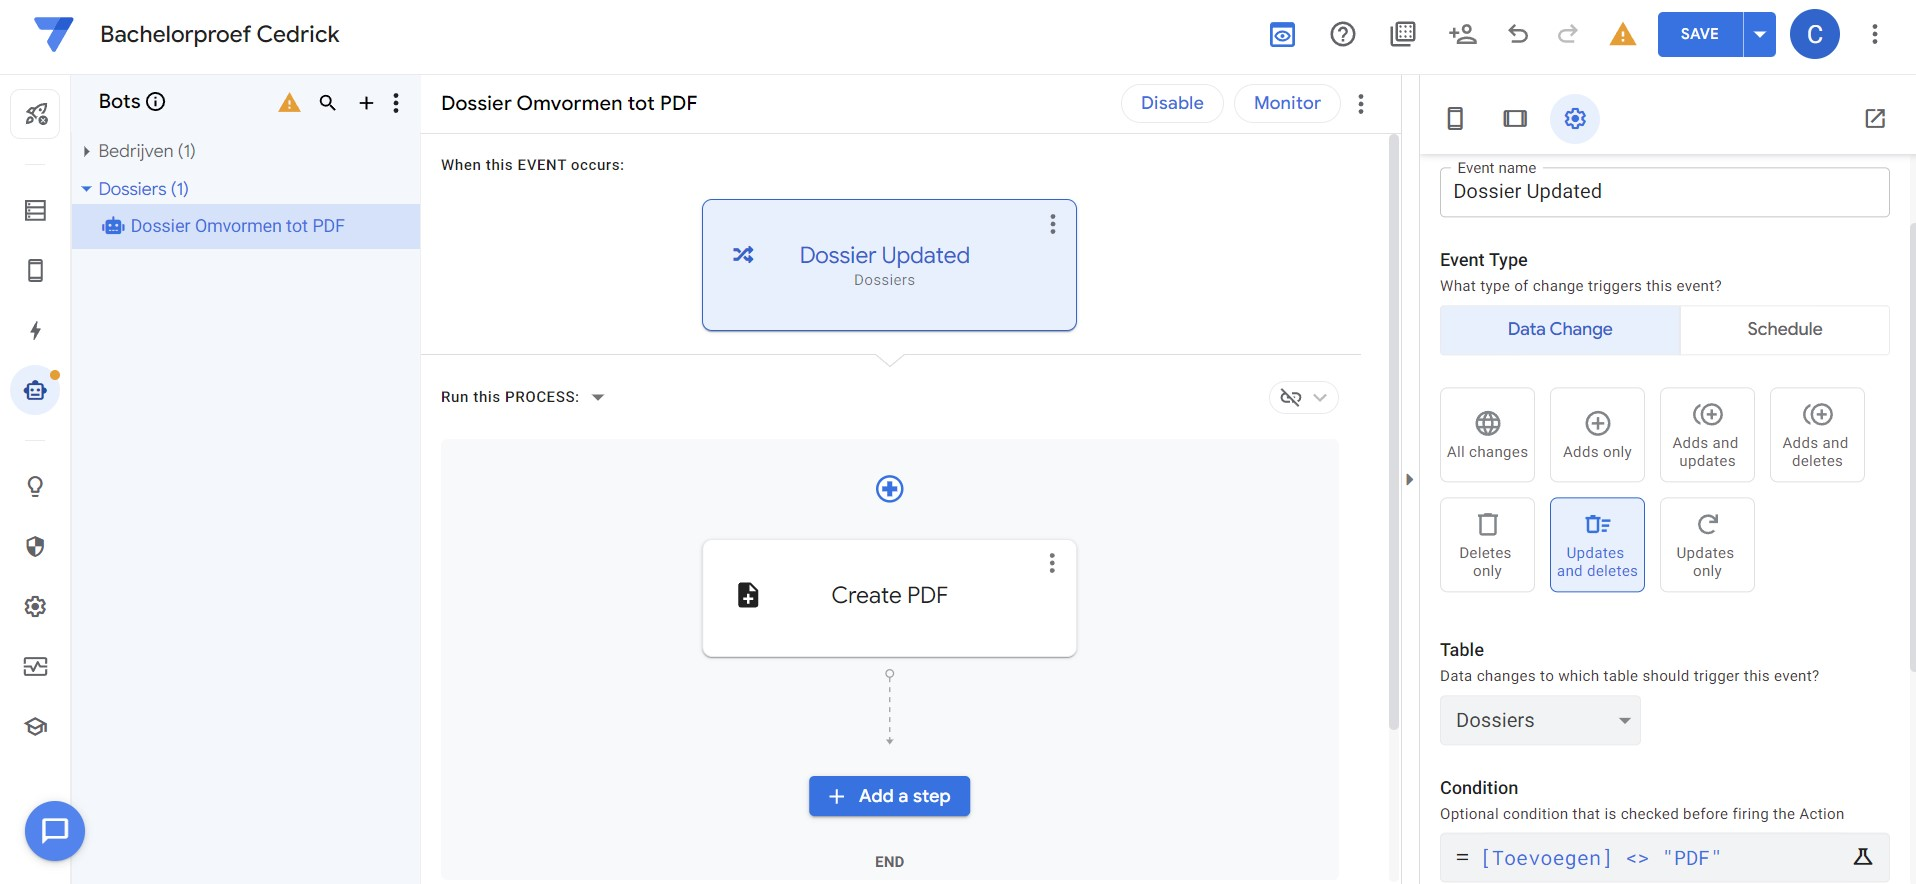
\includegraphics[width=0.85\textwidth]{methodologie/Appsheet_automations.jpg}
    \caption{Automatisaties of 'bots' in Appsheet.}
    \label{fig:meth_appsheet_automations}
\end{figure}


Uiteindelijk is het dus ook mogelijk om de use case uit te bouwen in Appsheet. Net zoals bij Airtable en Podio kunnen er relaties gelegd worden tussen de verschillende tabellen in de database. Verder is het feit dat calculaties op elk veld uitgevoerd kunnen worden een enorm pluspunt, toch is hun functionaliteit veel beperkter dan de calculatievelden in Podio. Op gebied van gebruikerservaring presteerde Appsheet het minst goed, er waren in het algemeen de meeste klikken\footnote{drie tot vijf} en stappen nodig om een doel te bereiken. Daarnaast waren er ook nog extra klikken nodig, zoals het synchroniseren van de database schema's tussen de het applicatie- en databasegedeelte en het heen en weer gaan tussen de twee delen. Desondanks het feit dat de UI van Appsheet duidelijk opgesteld is, kan ze als onoverzichtelijk overkomen op kleinere schermen, omdat alles dan meer op elkaar gezet wordt en er veel met scrollbars gewerkt moet worden. Ten slotte zijn er ook enkele problemen voorgekomen tijdens het uitwerken van de use case. Vaak waren dit synchronisatie problemen tussen de applicatie en de ingevulde formules. \\
